%&<tex>
\documentclass[notheorems,xcolor=dvipsnames]{beamer}
\usetheme{Rochester}
%\usefonttheme{serif}


%\usepackage[hmargin=2.5cm, vmargin=2cm]{geometry}
\usepackage{amssymb, mathtools, yhmath, graphicx}
\usepackage[most]{tcolorbox}
%\usepackage{fontspec, type1cm, titlesec, titling, fancyhdr, tabularx}
%\usepackage{unicode-math}
\usepackage{float}
\usepackage{transparent}

%\usepackage{eulervm}

\usepackage{xpatch}
%\usepackage[abbreviations, per-mode=symbol]{siunitx}
\usepackage[CheckSingle, CJKmath]{xeCJK}
\usefonttheme{professionalfonts}
\usepackage{ccfonts}
%\usepackage{CJKulem}
%\usepackage{enumitem}
\usepackage{tikz}
\usepackage{minted}
\setminted{fontsize=\footnotesize, linenos, frame=lines}
%\usemintedstyle{monokai}
%\usepackage{circuitikz}
%\setCJKmainfont[BoldFont=cwTex Q Hei]{cwTex Q Ming}
%\setCJKsansfont[BoldFont=cwTex Q Hei]{cwTex Q Ming}
%\setCJKmonofont[BoldFont=cwTex Q Hei]{cwTex Q Ming}
\setCJKmainfont{Source Han Sans TW}

\def\normalsize{\fontsize{12}{18}\selectfont}
\def\large{\fontsize{14}{21}\selectfont}
\def\Large{\fontsize{16}{24}\selectfont}
\def\LARGE{\fontsize{18}{27}\selectfont}
\def\huge{\fontsize{20}{30}\selectfont}

%\titleformat{\section}{\bf\Large}{\arabic{section}}{24pt}{}
%\titleformat{\subsection}{\large}{\arabic{subsection}.}{12pt}{}
%\titlespacing*{\subsection}{0pt}{0pt}{1.5ex}

%\usepackage{parskip}
%\parindent=24pt
%\parskip=1em

\makeatletter
%\newcommand{\myRelbar}{%
    %{\Rightarrow}%
    %\llap{\color{black}{\rule[-0.2ex]{1.1ex}{2ex}}}%
    %\kern-1.5ex}
%\let\saveLongrightarrow\Longrightarrow
\renewcommand{\Longrightarrow}{%
    %%\mathrel{\rlap{$\m@th\myRelbar\myRelbar$}%
    %%\phantom{{\saveLongrightarrow}}%
    %%\llap{$\m@th\Rightarrow$}}}
\Relbar\joinrel\mathrel{\raisebox{0.095ex}{\scalebox{0.85}{${\Rightarrow}$}}}
}
\makeatother


\newcommand{\img}{\mathsf{i}}
\newcommand{\ex}{\mathsf{e}}
\newcommand{\dD}{\mathrm{d}}
\newcommand{\dI}{\,\mathrm{d}}

\newcommand\abs[1]{\left\lvert #1 \right\rvert}
\newcommand{\ord}{\mathcal{O}}
\newcommand*{\defeq}{\triangleq}

\newcommand*{\bZ}{\mathbb{Z}}

\theoremstyle{definition}
\newtheorem{theorem}{定理}
\newtheorem{lemma}{引理}
\newtheorem{problem}{例題}
\newtheorem{definition}{定義}

\newenvironment{missue}{%
\setbeamercolor{block title}{bg=ForestGreen,fg=white}
\setbeamercolor{block body}{bg=blue!20!green!20,fg=black}
\begin{block}{\centering 問題}}{\end{block}}

\newenvironment{exercise}{%
\setbeamercolor{block title}{bg=ForestGreen,fg=white}
\setbeamercolor{block body}{bg=blue!20!green!20,fg=black}
\begin{block}{習題}}{\end{block}}

\renewenvironment{proof}{%
\begin{tcolorbox}[frame empty] {\bf 證明:}\ }{\end{tcolorbox}}

\setbeamercovered{transparent}
%\usefonttheme[onlymath]{serif}
%\settowidth{\leftmargini}{\usebeamertemplate{itemize item}}

%\makeatletter
%\patchcmd\beamer@@tmpl@frametitle{\insertframetitle}{\insertsection-\insertframetitle}{}{}
%\makeatother

\title{IOI-camp lecture Math}
\author{Meteor}

\renewcommand*{\emph}[1]{{\bf #1}}

\begin{document}

\begin{frame}
  \titlepage
\end{frame}

\section{Introduction}

\begin{frame}{\secname}
  程式競賽中的數學:

  \begin{itemize}
    \setlength{\itemindent}{2em}
    \item<2-> 數學知識
    \item<3> 數學想法
  \end{itemize}
\end{frame}

\begin{frame}[t]{\secname \ -- 數學知識例子}
  \begin{problem}[平方國的平方幣, TIOJ 1349]
    給你一個正整數 $n$,請找出最小的 $k$,使得存在 $k$ 個平方數 $a_1^2, a_2^2, \cdots, a_k^2$
    使得 $\sum a_i^2 = n$ 。($n \leq 10^7$)
  \end{problem}

  \begin{itemize}
    \item<2-> 一個很極端的「結論題」。
    \item<3-> 所有正整數都可以寫成 $4$ 個平方數的和 (Lagrange 1770)。
    \item<4-> 太結論也不是很有趣……
  \end{itemize}
\end{frame}

\begin{frame}[t]{\secname \ -- 數學知識例子 2}
  \begin{problem}[Taxes, Codeforces 735D]%
    在一個很古怪的國家,如果你賺了 $x$ 元,你就要繳 $d$ 塊錢的稅,其中 $d$ 是 $x$ 的因數且小於
    $n$ 裡最大的一個。

    \medskip
    現在有一個人賺了 $n$ 元,他想把 $n$ 拆成 $n = n_1 + n_2 + \cdots + n_k$ 然後 $n_i$ 各自繳稅,
    請問他最多可以逃過多少稅?($n \leq 2 \times 10^9$)
  \end{problem}

  \begin{itemize}
    \item<2-> Goldbach's conjecture: 大於 $2$ 的偶數都可以寫成兩個質數的和。
  \end{itemize}
\end{frame}

\begin{frame}[t]{\secname \ -- 數學想法例子}
  但大部份還是屬於「數學想法」的問題。

  \pause
  \medskip
  \begin{problem}[2015 ICPC Daejeon regional pE]
    給你一堆數列 $a_1, a_2, \cdots, a_n$,你要找一個排列 $\sigma$,使得
    \[ \max \Big(
      \abs{a_{\sigma(1)} - a_{\sigma(2)}},
      \abs{a_{\sigma(2)} - a_{\sigma(3)}}, \cdots,
      \abs{a_{\sigma(n)} - a_{\sigma(1)}}
      \Big) \]
    最小。 ($n \leq 10^4$)
  \end{problem}

  \pause
  \begin{definition}
    一個大小為 $n$ 的\emph{排列}是一個從 $[1, n]$ 打到自己的一一對應函數。
  \end{definition}
\end{frame}

\begin{frame}[t]{\secname \ -- 數學想法例子}
  解題四部曲:
  \pause

  \begin{enumerate}[<+->]
    \item 嘗試、觀察:在計算紙上多試試
    \item 神猜結論
    \item {\color{gray} (稍微)}證明
    \item 寫 code
  \end{enumerate}
  \pause

  \bigskip
  亂講的,多半要臨機應變,見招拆招。
\end{frame}

\begin{frame}[t]{\secname \ -- 數學想法例子}
  \begin{enumerate}
    \item 嘗試、觀察
    \item 神猜結論
  \end{enumerate}
  \pause

  \begin{figure}
    \centering
    \only<+>{
    \begin{tikzpicture}[scale=0.8]
      \draw[-latex, thick] (0, 0) -- (10, 0);
      \foreach \x [count=\i] in {0.5, 2, 4, 6, 8} {
        \fill (\x, 0) node (\i) {} circle (1.5mm);
      }
      \node at (0, 0) {};
      \draw (1) edge[bend left=50, -latex, thick] (2);
      \draw (2) edge[bend left=50, -latex, thick] (3);
      \draw (3) edge[bend left=50, -latex, thick] (4);
      \draw (4) edge[bend left=50, -latex, thick] (5);
      \draw (5) edge[bend left=50, -latex, thick] (1);
      \node at (5, -3) {應該不是…};
    \end{tikzpicture}
    }

    \only<+>{
    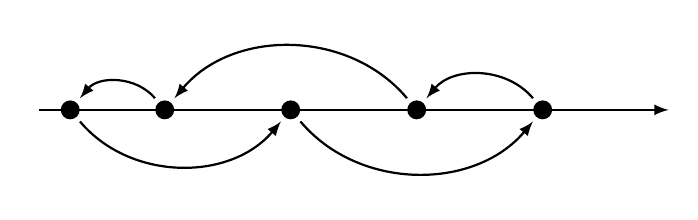
\begin{tikzpicture}[scale=0.8]
      \draw[-latex, thick] (0, 0) -- (10, 0);
      \foreach \x [count=\i] in {0.5, 2, 4, 6, 8} {
        \fill (\x, 0) node (\i) {} circle (1.5mm);
      }
      \node at (0, 0) {};
      \draw (2) edge[bend right=50, -latex, thick] (1);
      \draw (1) edge[bend right=50, -latex, thick] (3);
      \draw (3) edge[bend right=50, -latex, thick] (5);
      \draw (5) edge[bend right=50, -latex, thick] (4);
      \draw (4) edge[bend right=50, -latex, thick] (2);
    \end{tikzpicture}
    }

    \only<+>{
    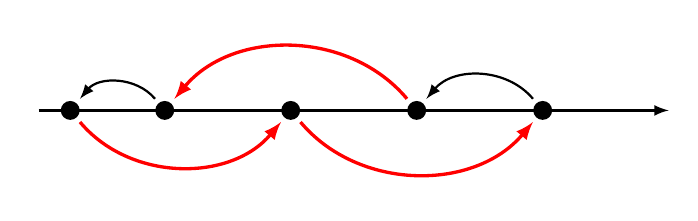
\begin{tikzpicture}[scale=0.8]
      \draw[-latex, thick] (0, 0) -- (10, 0);
      \foreach \x [count=\i] in {0.5, 2, 4, 6, 8} {
        \fill (\x, 0) node (\i) {} circle (1.5mm);
      }
      \node at (0, 0) {};
      \draw (2) edge[bend right=50, -latex, thick] (1);
      \draw (1) edge[bend right=50, -latex, very thick, red] (3);
      \draw (3) edge[bend right=50, -latex, very thick, red] (5);
      \draw (5) edge[bend right=50, -latex, thick] (4);
      \draw (4) edge[bend right=50, -latex, very thick, red] (2);
    \end{tikzpicture}
    }
  \end{figure}
\end{frame}

\begin{frame}[t]{\secname \ -- 數學想法例子}
  \begin{enumerate}
    \setcounter{enumi}{2}
    \item 證明
  \end{enumerate}

  \begin{figure}
    \centering
    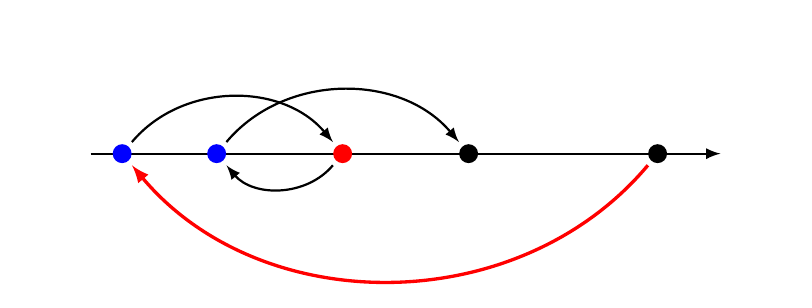
\begin{tikzpicture}[scale=0.8]
      \useasboundingbox (-1, -2) rectangle (11, 2);
      \draw[-latex, thick] (0, 0) -- (10, 0);
      \fill[red] (4, 0) node (1) {} circle (1.5mm);
      \fill (6, 0) node (2) {} circle (1.5mm);
      \fill<+-> (9, 0) node (3) {} circle (1.5mm);
      \fill<+->[blue] (2, 0) node (4) {} circle (1.5mm);
      \draw<.-> (1) edge[bend left=50, -latex, thick] (4);
      \draw<.-> (4) edge[bend left=50, -latex, thick] (2);
      \fill<+->[blue] (0.5, 0) node (5) {} circle (1.5mm);
      \draw<.-> (5) edge[bend left=50, -latex, thick] (1);
      \draw<.-> (3) edge[bend left=50, -latex, very thick, red] (5);
    \end{tikzpicture}
  \end{figure}
\end{frame}

\begin{frame}[t, fragile]{\secname \ -- 數學想法例子}
  \begin{enumerate}
    \setcounter{enumi}{3}
    \item 寫 code
  \end{enumerate}

  \begin{minted}{cpp}
sort(begin(a), end(a));
int ans = 0;
for (int i=0; i<n-2; i++)
  ans = max(ans, a[i+2] - a[i]);
cout << ans << endl;
  \end{minted}
  \pause

  \bigskip
  Very easy! --- 有時漂亮的結論就會有很短的程式碼。
\end{frame}

\begin{frame}{\secname}
  相同的題目就不會在出現第二次了。
  \pause

  \bigskip
  \alert{但用類似想法的題目有可能會在出現!}

  \pause
  \smallskip
  要有舉一反三的能力!
\end{frame}

\begin{frame}[t]{\secname \ -- 數學想法例子 2}
  \begin{problem}[2016 NTU PK pF]
    給你一堆數列 $a_1, a_2, \cdots, a_n$,你要找一個排列 $\sigma$,使得
    \[ \min_{1 \leq i < n} \abs{a_{\sigma(i)} - a_{\sigma(i+1)}} \]
    最大。 ($n \leq 2 \times 10^5$)
  \end{problem}
  \pause

  \medskip
  我們先想 $n$ 是\alert{偶數}的 case。
\end{frame}

\begin{frame}[t]{\secname \ -- 數學想法例子 2}
  \begin{enumerate}
    \item 嘗試、觀察
    \item 神猜結論
  \end{enumerate}

  \begin{figure}
    \centering
    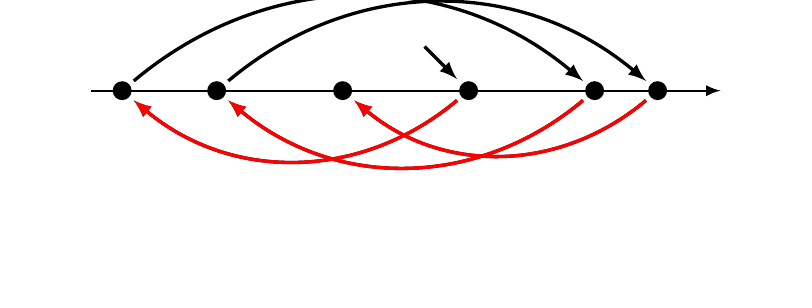
\begin{tikzpicture}[scale=0.8]
      \useasboundingbox (-1, -3) rectangle (11, 1);
      \draw<+->[-latex, thick] (0, 0) -- (10, 0);
      \foreach \x [count=\i] in {0.5, 2, 4, 6, 8, 9} {
        \fill (\x, 0) node (\i) {} circle (1.5mm);
      }
      \draw<+> (4) edge[bend left=40, -latex, very thick] (1);
      \draw<.-> (1) edge[bend left=40, -latex, very thick] (5);
      \draw<.> (5) edge[bend left=40, -latex, very thick] (2);
      \draw<.-> (2) edge[bend left=40, -latex, very thick] (6);
      \draw<.> (6) edge[bend left=40, -latex, very thick] (3);
      \draw<.-> (4) ++ (-0.7, 0.7) edge[-latex, very thick] (4);

      \draw<+-> (4) edge[bend left=40, -latex, very thick, red] (1);
      \draw<.-> (5) edge[bend left=40, -latex, very thick, red] (2);
      \draw<.-> (6) edge[bend left=40, -latex, very thick, red] (3);
    \end{tikzpicture}
  \end{figure}
\end{frame}

\begin{frame}[t]{\secname \ -- 數學想法例子 2}
  \begin{enumerate}
    \setcounter{enumi}{2}
    \item 證明
  \end{enumerate}

  \begin{figure}
    \centering
    \begin{tikzpicture}[scale=0.8]
      \useasboundingbox (-1, -3) rectangle (11, 1);
      \draw<+->[-latex, thick] (0, 0) -- (10, 0);
      \foreach \x [count=\i] in {0.5, 9} {
        \fill (\x, 0) node (\i) {} circle (1.5mm);
      }
      \foreach \x [count=\i] in {2, 4, 6, 8} {
        \fill[red] (\x, 0) node (\i) {} circle (1.5mm);
      }

      \draw[latex-latex] (2, -.5) -- (8, -.5);
      \draw (2, -.8) -- (2, -.2);
      \draw (8, -.8) -- (8, -.2);
    \end{tikzpicture}
  \end{figure}
\end{frame}

\begin{frame}{\secname \ -- 數學想法例子 2}
  \begin{exercise}
    請完成奇數的情況。
  \end{exercise}
\end{frame}

\section{數論}

\begin{frame}[t,fragile]{\secname}
  \begin{problem}[An Easy Problem, NTUJ 1423]
    給你等式 $a^b \equiv c \pmod{d}$ 中的其中 $3$ 個,請找出剩下的一個。
  \end{problem}
  \pause

  \bigskip
  \begin{enumerate}
    \item $a^b \equiv \raisebox{-.2mm}{\text{?}} \pmod{d}$: 快速冪,$\ord(\log b)$。
  \end{enumerate} \vspace{-1em} \pause
  \begin{minted}{cpp}
int fastpow(int a, int b, int m) {
    if (!b) return 1%m;
    int ret = fastpow(a*a%m, b/2, m);
    if (b&1) (ret *= a) %= m;
    return ret;
}
  \end{minted}
\end{frame}

\begin{frame}[t]{\secname}
  \begin{enumerate}
    \setcounter{enumi}{1}
    \item $a^b \equiv c \pmod{\text{?}}$ \pause $\implies \raisebox{-.2mm}{?} \mid a^b - c$ \pause
      \vspace{1em}
    \item<+-> $a^{\text{?}} \equiv c \pmod{p},\, p \text{ prime}$: $\ord\big( \sqrt{p} \big)$,有點難了。

      \[ a^{xk + y} \equiv c \pmod{p} \iff a^{xk} \equiv c a^{-y} \pmod{p} \]

      \begin{missue}<+->
        \centering
        怎麼求出 $a^{-y} \bmod p$?
      \end{missue}
  \end{enumerate}
\end{frame}

\begin{frame}{\secname}
  我們先離題一下。
  \pause

  \medskip
  數學上喜歡把東西抽象化,只留下「本質」,去掉多餘的東西。
  \pause

  \medskip
  \begin{missue}<+->
    \centering
    運算的「本質」是什麼?
  \end{missue}
\end{frame}

\begin{frame}{\secname \ -- 群}
\begin{definition}[群] 一個\emph{群}由一個集合 $G$ 和一個運算 $\cdot$ 構成,滿足
  \begin{itemize}
    \item 運算 $\cdot$ 是一個函數 $(G, G) \to G$,也就是說 $x \cdot y \in G$。
    \item 有\emph{結合律}:$(x \cdot y) \cdot z = x \cdot (y \cdot z)$
    \item 存在一個特別的元素 $1$ 叫作\emph{單位元},滿足 $1 \cdot x = x \cdot 1 = x$。
    \item 對每一個 $x$ 存在 $x^{-1} \in G$ 叫作\emph{反元素},滿足 $x \cdot x^{-1} = x^{-1} \cdot x = 1$。
  \end{itemize}
\end{definition}
\end{frame}

\begin{frame}[t]{\secname \ -- 群的例子}
  \begin{itemize}
    \item 整數對於加法 $(\bZ, +)$ 是一個群。
    \item 旋轉是一個群,如 $0, \pi/2, \pi, 3\pi/2$。
    \item 模 $m$ 下的加法,寫作 $\bZ / m\bZ$。
    \item 一個元素生成的群 $\langle a \rangle \defeq \{ a^k \mid k \in \bZ \}$,我們把這種群叫作%
      \emph{循環群}。
  \end{itemize}

  \begin{missue}
    \centering
    模 $m$ 下的乘法 $(\bZ / m\bZ)^{\times}$ 是一個群嗎?
  \end{missue}
\end{frame}

\begin{frame}[t]{\secname \ -- $(\bZ / m\bZ)^{\times}$}
  剛剛那樣問並不精確,關鍵應是模 $m$ 下哪些元素有反元素?\pause

  \medskip
  $2$ 在模 $12$ 下就沒有反元素。 \pause

  \[ xy \equiv 1 \pmod{m} \pause\implies xy = mt' + 1 \pause\implies xy + mt = 1 \]

  \begin{missue}<+->
    \centering
    給定 $a, b, c$,$ax + by = c$ 什麼時候有整數解 $(x, y)$?
  \end{missue}
\end{frame}

\begin{frame}[t, fragile]{\secname \ -- $ax + by = c$}
  \begin{theorem} \vspace{-1em}
    \[a \bZ + b \bZ = \gcd(a, b) \bZ \]
  \end{theorem}\pause

  $a \bZ + b \bZ \supseteq \gcd(a, b) \bZ $:
  \begin{minted}{cpp}
pair<int, int> extend_gcd(int a, int b) {
    if(b == 0) return {1, 0};
    else {
        int k = a/b;
        pair<int, int> xy = gcd(b, a%b);
        return {xy.second, xy.first - k * xy.second};
    }
}
  \end{minted}
\end{frame}

\begin{frame}[t]{\secname \ -- $(\bZ / m\bZ)^{\times}$}
  \begin{lemma} \vspace{-1em}
    \[ x \in (\bZ / m\bZ)^{\times} \iff \gcd(x, m) = 1 \]
  \end{lemma}
  \pause

  \begin{proof}
    \begin{align*}
      \only<2->{xy \equiv 1 \ (\mathrm{mod}\ m) \text{ 有解} & \iff xy + mt = 1 \text{ 有解} \\}
      \only<3->{& \iff \gcd(x, m) = 1}
    \end{align*}
  \end{proof}
\end{frame}

\begin{frame}[t]{\secname \ -- $(\bZ / m\bZ)^{\times}$}
  \begin{missue}
    $(\bZ / m\bZ)^{\times}$ 有多少元素?也就是 $[1, n]$ 中有幾個數和 $n$ 互質?
  \end{missue}
  \pause

  \begin{theorem}[Euler $\varphi$ 函數]
    $\varphi(n)$ 表示 $[1, n]$ 有幾個數和 $n$ 互質,則如果 $n = p_1^{\alpha_1} p_2^{\alpha_2} \cdots p_k^{\alpha_k}$,則
    \[ \varphi(n)
      = n \left( 1 - \frac1{p_1} \right) \left( 1 - \frac1{p_2} \right) \cdots \left( 1 - \frac1{p_k} \right)\]
  \end{theorem}

\end{frame}

\begin{frame}[t]{\secname \ -- 子群}
  \begin{definition}
    如果 $H \subseteq G$ 且 $H$ 中任兩個元素的乘積、任一個元素的反元素還在 $H$ 裡,我們就說 $H$ 是 $G$ 的\emph{子群}。
  \end{definition}

  \begin{itemize}
    \item 所有偶數 $2 \bZ$ 對於加法是 $\bZ$ 的子群。
    \item $H \defeq \{\bar{1}, \bar2, \bar4\}$ 對於乘法是 $\bZ / 7\bZ$ 的子群。
  \end{itemize}
\end{frame}

\begin{frame}[t]{\secname \ -- Lagrange's Theorem}
  \begin{theorem}[Lagrange's theorem]
    如果 $H$ 是 $G$ 的子群,則 $\abs{G} = \abs{G / H} \abs{H}$,因此有 $\abs{H} \bigm\vert \abs{G}$。
  \end{theorem}
  \pause

  \bigskip
  \begin{theorem}[Euler's theorem] \vspace{-1em}
    \[ a^{\varphi(m)} \equiv 1 \pmod{m} \]
  \end{theorem}
\end{frame}

\begin{frame}[t]{{\secname} -- Euler's Theorem}
  \begin{proof} \\
    如果 $n$ 是最小的正整數使得 $a^n \equiv 1 \pmod{m}$,那
    $H \defeq \langle a \rangle = \{1, a, a^2, \cdots, a^{n-1}\}$ 有 $n$ 個元素。

    \smallskip
    由 Lagrange's theorem,$n \bigm\vert \abs{(\bZ / m\bZ)^{\times}} = \varphi(m)$,可令 $\varphi(m) = nk$,
    因此 $a^{\varphi(m)} = a^{nk} \equiv 1 \pmod{m}$。
  \end{proof}

  \begin{lemma}<+->
    \vspace{-1em}
    \[ \gcd(a, m) = 1 \implies a^{-1} \equiv a^{\varphi(m)-1} \pmod{m} \]
  \end{lemma}
\end{frame}

\begin{frame}{{\secname} -- Tonelli-Shanks algorithm}
  回到一開始的題目:
  \begin{enumerate}
    \setcounter{enumi}{3}
    \item $\raisebox{-.2mm}{\text{?}}^{b} \equiv c \pmod{p},\, p \text{ prime}$。
  \end{enumerate}
  \pause

  \bigskip
  先看 $b = 2$ 的情況。
  \begin{problem}[Square Roots in a Finite Group, 2013 大專院校 pJ]
    給定一個質數 $p$ 和 $a$,請求出 $x^2 \equiv a \pmod{p}$ 的解 $x$ 或輸出無解。
    ($a, p < 2^{31}$)
  \end{problem}
\end{frame}

\begin{frame}[t]{{\secname} -- Tonelli-Shanks algorithm}
  當時這一題有給一個小題示。

  \begin{enumerate}
    \item 把 $p-1$ 寫作 $p-1 = 2^s m$,其中 $m$ 是奇數。
    \item 找一個 $b$ 使得 $x^2 \equiv b \pmod{p}$ 無解。
    \item 令 $b \gets b^m,\, x \gets a^{(m+1)/2},\, t \gets a^m$,\\
      可以驗證 $x^2 \equiv at \pmod{p}$。
    \item 想辦法把 $t$ 調成 $1$ 你就獲勝了。
  \end{enumerate}
  \pause

  \begin{figure}
    \centering
    \includegraphics[width=0.45\textwidth]{figure/what.jpg}<+->
  \end{figure}
\end{frame}

\begin{frame}{{\secname} -- 原根}
  要有一點先備知識。\pause

  \bigskip
  \begin{theorem}
    \vspace{-1em}
    \[ (\bZ / m\bZ)^{\times} \text{ 是一個循環群} \iff m = 1, 2, 4, p^k, 2p^k \]
  \end{theorem}
  \pause

  \bigskip
  \begin{definition}
    如果 $(\bZ / m\bZ)^{\times} = \langle a \rangle$,我們就說 $a$ 是模 $m$ 下的\emph{原根}。
  \end{definition}
\end{frame}

\begin{frame}{{\secname} -- 原根}
  舉個例子,$m = 11, a = 2$。
  \begin{table}
    \begin{tabular}{c||c|c|c|c|c|c|c|c|c|c}
      $\bZ / 10\bZ$
      & 0 & 1 & 2 & 3 & 4 & 5 & 6 & 7 & 8 & 9 \\
      \hline
      $(\bZ / 11\bZ)^{\times}$
      & 1 & 2 & 4 & 8 & 5 & 10 & 9 & 7 & 3 & 6 \\
    \end{tabular}
  \end{table}
  \pause

  \[
    \begin{array}{cccccl}
      2 & +      & 4 & \equiv & 6 & \pmod{10} \\
      \updownarrow & & \updownarrow & & \updownarrow & \\
      4 & \times & 5 & \equiv & 9 & \pmod{11} \\
    \end{array}
  \]
  \pause

  可定義 $\log_a$,如 $\log_2(9) = 6$。
\end{frame}

\begin{frame}{{\secname} -- Tonelli-Shanks algorithm}
  $p = 25,\ p-1 = 2^s \cdot m = 2^3 \cdot 3$ \\
  \visible<2->{ $\log(t) = \log(a^m) = m \log(a)$。}\visible<3->{如果 $x \gets b$,那 $t \gets b^2$。}
  \begin{figure}
    \centering
    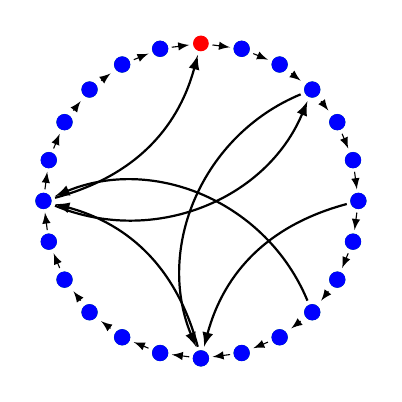
\begin{tikzpicture}
      \useasboundingbox (-2.2cm, -2.2cm) rectangle (2.2cm, 2.2cm);
      \fill[red] (90:2cm) node(0){} circle (1mm);
      \foreach \deg [count=\xi] in {75, 60,..., -255} {
        \fill (\deg:2cm) node(\xi){} circle (1mm);
        \pgfmathtruncatemacro{\hao}{mod(\xi,3)}
        \ifthenelse{\hao = 0}{
          \fill<2-5>[green] (\deg:2cm) node{} circle (1.02mm);
        }{ }
        \pgfmathtruncatemacro{\tsan}{mod(\xi,6)}
        \ifthenelse{\tsan = 0}{
          \fill<3-5>[blue] (\deg:2cm) node{} circle (1.04mm);
        }{ }
      }
      \foreach \xi [remember=\xi as \lastx (initially 0)] in {1,...,23}{ \draw[-latex] (\lastx) -- (\xi); }
      \draw[-latex] (23) -- (0);

      \foreach \xi [remember=\xi as \lastx (initially 6)] in {12, 18, 0} {
        \draw<4> (\lastx) edge[bend right, -latex, thick] (\xi);
      }

      \foreach \xi [remember=\xi as \lastx (initially 9)] in {18, 3, 12} {
        \draw<5> (\lastx) edge[bend right=45, -latex, thick] (\xi);
      }
    \end{tikzpicture}
  \end{figure}
\end{frame}

\begin{frame}[fragile]{{\secname} -- Tonelli-Shanks algorithm}
  \begin{minted}{cpp}
while (t != 1) {
    int k = 0, tp = t, tb = b;
    while (tp != 1) tp = (tp * tp) % p, k++;
    for (int i=0; i<s-k-1; i++) tb = (tb * tb) % p;
    x = x * tb % p;
    t = t * tb * tb % p;
}
  \end{minted}

\begin{exercise}
  把剩下的細節弄清楚!
\end{exercise}
\end{frame}


\end{document}

